\section{Introduction}
In large scale networks, as in Datacenters, the conception and set up of the network topology is usually challenging, bearing in mind not only the careful choice of software/hardware that must be done to satisfy accurately the specific requirements, but also how a compatibility among the hardware devices provided by different vendors can be reached. Nevertheless, this variety of hardware vendors could create further problems whenever a change in the network topology or addition of network functions must be made in the Datacenter. In the other hand, the classical approach of networking has always been about the hardware, given that networking devices are offered to customers pre-built to work in a specifc way, hence offering minimum flexibility to control and manipulate the technologies and protocols laying upon the hardware devices, depending on the customer’s and network’s situation. These two major limitations can often prove costly in terms of network’s performance, or at least can prevent major performance improvement in some situations. There is no better way to illustrate those potential improvements than an example. In a simple topology where many hosts are connecting to a router (modern router that can do also the switche’s role), let’s imagine a situation, where, for the sake of the argument, only two hosts are currently active, and have no interest in connecting to an external network, and want instead to exchange files between them using FTP. With the provided router, only a pre-determined range of the bandwidth can be given for these 2 hosts and for the FTP protocol as well. In an ideal situation, the majority of the bandwidth would be given for these 2 hosts and for the FTP exchange, since no other host is currently active, and also because the 2 hosts do not want to connect to an external network simultaneously. Hence the introduction of a new networking concept, SDN, where a (new type of) networking device can be controlled and manipulated independently from the technology that lays upon it, in order to improve the performance and increase the flexibily of the network. Obviously, the access to these devices and controlling them has to be done through a programming interface, and following some protocols, which explains the network being defined by software (and code). These details will be discussed in a later section. In spite of the flexibility that SDN can offer, the variety of hardware devices for the different networking functions (Firewalls, DNS,...) is proving to be highly consuming, especially in terms of energy, resulting therefore in higher costs. Another concept was introduced to resolve this limitation, NFV, which is basically about providing common hardware that can support many networking functions working upon it, economizing consequently consumption costs in a significant manner, and prove to be useful in the network’s topology complexity as well. These major concepts (SDN and NFV) and how they coexist to improve different aspects of networking will be discussed in more details in the next sections.
\newpage
\section{Network Functions' Virtualization}
The new solutions and options that came with the cloud computing and virtualization emergence were so efficient in terms of performance and costs, that it was hard to let the opportunity of introducing such concepts to the
networking field pass by, bearing in mind the profits that can be made in terms of cost and energy in that regard. Given that the virtualization concept is about maximizing the software/hardware independance, the main challenge in virtualizing networks was to provide a common hardware platform that can support running any networking technology upon it, and more importantly, that can also provide different networking functions, such as
DNS and physical Firewalls. Further problems also used to be encountered because of the hardware provided by different vendors, which meant finding issues such as the different drivers required for each device and whether these devices can coexist with devices that are provided by a different vendor. Beside the hardware’s complexity, issues emerged also on whether you can find the right
technicians to configure your datacenter, since each device requires its own expertise. All these problems lead eventually to higher costs in terms of time, maintenance, and money. With NFV, not only the complexity was reduced,
but it assured that it was sufficient to connect the device to a server to controll it in the most simplistic way, with no need to the specific’s device manual to configure it, which meant that even the expertise issues did no longer exist.
\section{Software Defined Networks}
The networking approach consisting of relying majorly on hardware, while being considered efficient to some extent, lacks some flexibility to adapt the available bandwidth depending on the user’s needs. In fact, the devices offered to customers leave barely the option to be functionnally controlled, and can only be accessed for configuration purposes. Therefore, it was of a prime
importance to provide a solution where the hardware can be manipulated flexibly, especially in large scale and complex networks, where the change of needs and maintenance emerege very frequently. Consequently, a new networking structure was suggested, where the hardware -The control plane- would only be needed for circuiting purposes and forwarding packets, while the forwarding plane (the controller), typically a server, is the ’brain’ of the network, that is to say, the part of the network responsible for routing and every software-related aspect of the network. Given this new architecture, even
large scale networks can be totally and flexibly controlled through programming interfaces. This approach does certainly offers numerous advantages as we can list below:
\begin{description}
\item[Direct Programmability] As previously explained, decoupling the control plane from the forwarding plane allows direct access to the network. Therefore, the forwarding plane becomes programmable.
\item[Agility] Abstracting the technology from the hardware makes the network dynamically adjustable and adapatable to the needs of the network’s administrator.
\item[Central Management] The centralization of the network’s intelligence in the controller, which makes the whole network manageable from servers.
\item[Vendors-Neutral] Managing the network through servers increase the independence of the network from the hardware and the vendors that provide them.
\end{description}
\section{Service Function Chains \cite{nano3}}
After explaining how advantageous both SDN and NFV can be for any network, with the former being more profitable in terms of software and technology, hence increasing the network’s flexibility, while the latter offering hardware-related advantages, given how it provides common hardware
platform that supports many networking fucntions laying upon it. However, network architects are always under obligation to combine all the networking solutions available in order not only to satisfy the requirements included in the customer’s specifications, but to accomplish the most balanced specification/cost ratio possible as well. The SDN/NFV combination can massively contirbute in reaching this balance. As explained before, SDN can increase the dynamic apsect of the network, thus improving its performance and maintenance. In the other hand, by providing common hardware able to support many networking functions, hardware and energy costs are signf-
icantly reduced. Eventually, this combination produces low complexity, high maintenance ability, and improved performance adaptability: Direct impacts of abstraction and virtualization.\\
More importantly, the combination of these two fundamental concepts gave birth to a new form of networking, where network functions are presented as an ordered set (chain) of basic service functions, increasing therefore the flexibility of the networking functions and their adaptability to the network’s changing requirements. In the next parts of this work, we define Service Function Chains as well as its main components and how they interact.
\subsection{Definition}
SFC can be defined as a concept that enables the creation of composite networking services (Service Functions) that are strictly oredered, in order to apply them to packets/frames matching the rules of these Service Functions
(Classification). SFC also offers a method of deployment for SFs, in which the order of the service functions can be dynamically changed and independent of its underlying topology using simply the exchanged messages.
\subsection{Components}
\vspace*{0.5cm}
\textbf{Service Function} A specific function that processes incoming packets following predefined rules. Functions can be involved in the delivery of added-value services. A non-exhaustive list of abstract service functions includes: firewalls, Deep Packet Inspection, NAT...\\
\\
\textbf{Service Function Forwarder} A logical component that forwards traffic to the connected
service functions according to information carried in the SFC
encapsulation. It does also handle traffic coming back from the
Service Functions.\\ 
\\
\textbf{Metadata} Exchanged context information among the different SFC components.\\
\\
\textbf{Service Function Path} a
constrained specification of where packets assigned to a certain
service function path must go. Specific details declaration is not mandatory. While in some cases the different Service Functions to be visited are fully specified, we can always maintain a certain level of abstraction in some other cases.\\
\\
\textbf{SFC Encapsulation} The SFC encapsulation  provides identification for SFP. It is equally  used by the SFC-aware functions. In addition, the SFC encapsulation carries metadata.\\
\\
\textbf{Rendered Service Path}  The different SFs and SFFs visited by a packet in the network.\\
\\
\textbf{SFC-Enabled Domain} A network or region of a network where SFC is implemented.\\
\\
\textbf{SFC Proxy} Logical component that removes and inserts SFC encapsulation on behalf of an     SFC-unaware service function.
\subsection{Architecture}
\vspace*{0.5cm}
An SFC architecture does usually have to satisfy a set of principles in order to ensure using the SFC efficiently.\\
\\
\textbf{Topological Independence} 
The deployment SFs or SFCs does not require any changes in the underlay network forwarding topology.\\
\\
\textbf{Plane Separation} The packet handling operations should ne be confused with the the dynamic realization of the Service Forwarding Paths.\\
\\
\textbf{Classification} A specific SFP is responsible for any packet matching a specific rule.\\
\\
\textbf{Shared Metadata} Metadata/context data can be shared amongst Service Functions and classifiers, between SFs, and between external systems and SFs. Metadata could be used to provide and share the result of classification (that occurs within the SFC-enabled domain, or external to it) along an SFP.\\
\\ 
\textbf{Service Definition Independence} The SFC architecture does not depend on the details of SFs themselves.\\
\\
\textbf{SFC Independence} The creation, modification, or deletion of an SFC has no impact on other SFCs. The same is true for SFPs.\\
\\
\textbf{Heterogneous control/policy Points} The architecture allows SFs
to use independent mechanisms to
populate and resolve local policy and  local classification criteria.\\
\\
These architecture principles should be applied to the  different planes composing an SFC network. The environment associated to SFC is mainly separated into four main planes:\\
\\
\textbf{The Control Plane} mainly responsible for controlling and configuring the SFC related components. It should be noted that the control plane does only concern a subset of the parameters and facilities associated to the SF.\\
\\
\textbf{The Management Plane} it serves in allocating resources to the various SF and eventually active the various SF components. Management operations would consist in setting the number of CPU, memory bandwidth associated to the SFs as well as specific configuration parameters of the SFC components. Unlike the control plane, the management plane defines a large number of paramaters related to the SFC components configuration.\\
\\
\textbf{The Data Plane} consists in all SF components as well as the data exchanged between the SF components. Communications between SF components includes the packet themselves, their associated metadata, the routing logic or SF
logic. The SFC Data Plane can also be seen as all the elements that interact with a packet provided by an end user.\\
\\
\textbf{The SFC Tenant’s Users Data Plane} consists in the traffic data provided by the different users of the tenants. When a user is communicating with a server or another user, eventually from another administrative domain, the communication belongs to
the SFC Tenant’s Users Data Plane whenever packets are provided by the server or by the user.\\
\\
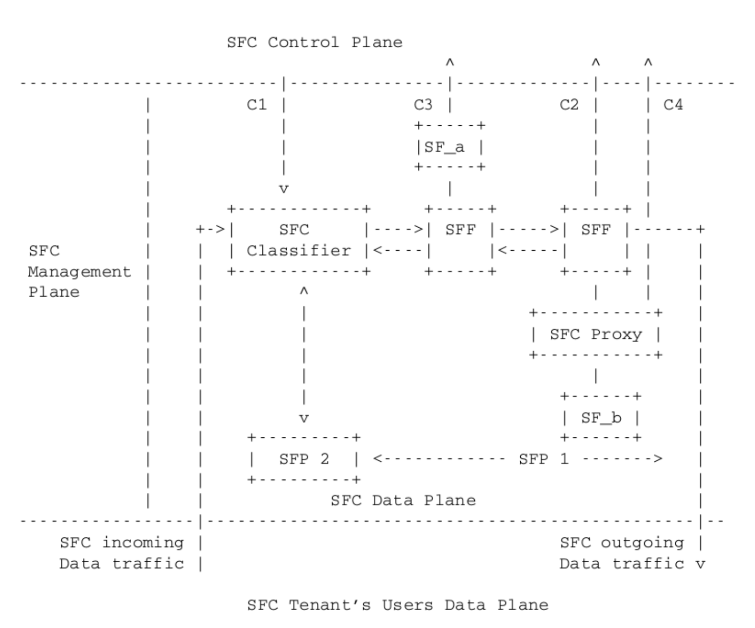
\includegraphics[scale=0.45]{sfc1}
\\
\\
\section{SFC Security Concerns Overview \cite{nano4}} 
The essential infrastructure required for the deployment of SFC is usually provided by a Cloud Provider. This infrastructure does include dedicated hardware serving a specified network function. The network function served by the dedicated hardware is the actual Service Function. If the SFC domain is not private to the company, the infrastructure and the dedicated hardwrare that it contains is often shared by multiple tenants. In some other cases, a local proxy does transparently redirect the local SFC network to an external SFC domain outside the local boundaries of the local infrastructure. Each SFC Tenant is responsible of its domain, that is to administrate or provision the necessary resource and control all its SFC element (e.g: defining SFC Paths, configuring the elements...). An SDN controller is responsible for the coordination of the SFC elements.\\
As for the security requirements for an SFC domain, they aim to protect the deployed SFC architecture from attacks. Even in a private SFC deployment, where SFC components are considered to be in a trusted environment, inside attacks are still possible (e.g. inside attacker sniffing the SFC metadata, sending spoofed packets...). The evolution of the local architecture could require, at some point, interconnecting with a third party SF/SFF, which puts the initial domain basically outside of the local (private) domain. Multitenancy also does represent a security concern, due to the fact of sharing an SFC platform. Unless the tenants are strongly isolated (physically or logically), different networks may share a common SFF, and one tenant may update the SFP of the other tenant. Such misconfiguration has similar impact as a redirecting attack.\\
The threats in this work are analysed in each plane. Even if the architecture is divided into many planes, so that the interactions can be limited and controlled, but these interactions still exist and so may be used by an attacker. As a result, for each plane, the threat analysis is performed by analysing the vulnerabilities present within each plane, as well as those performed via the other planes. We focus mainly on the threats faced by the Data Plane.\\
Attacks may be performed from inside the SFC Data Plane or from outside the SFC Data plane. Therefore, the attacker is in at least one of the following planes: SFC Control Plane, SFC Management Plane or SFC Tenants’ Users Plane.\\
\\
\textbf{Attacks performed from the SFC Control Plane}
Vulnerabilites can be found basically in the interfaces used for communication between the SFC Control Plane and the SFC Data Plane. These interfaces are responsible for updating the classification rules for the SFC classifier, updating forwarding decisions for SFFs and updating SFs/SFC proxys internal state. An attacker may change the SFC Classifier classification and
completely modify the services provided by the SFC. This could result in avoiding control over the tenant's traffic.\\
\\
\textbf{Attacks performed from the SFC Management Plane}
This type of attacks are basically similar to the previous type, with the only difference being that the SFC Management Plan provides usually a greater control of the SFC component that the SFC Control Plane.\\
\\
\textbf{Attacks performed from the SFC Data Plane} Given that an attacker has taken control of an SFC component, various types of attacks can be performed, such as modification of the traffic, performing onpath attacks, generating additionnal traffic to create heavy load situations. On the other hand, The traffic within the SFC Data Plane is composed of multiple
layers: the transport layer, the SFC encapsulation layer and the SFC payload layer. As a result, attacker may use the traffic to perform attacks at various layers.\\
\\
\\
\\
\textbf{1. Attacks performed at the transport layer}\\
\\
Mainly related to the illegitimate SFC traffic that could be provided to the SF. A malicious node that is not expected to communicate with that SF may inject packets into the SFC, That may eventually spoof the IP address of legitimate SF, so the receiving SF may not be able to detect the packet is not legitimate.\\
\\
\textbf{2. Attacks performed at the SFC encapsulation/payload layer}\\ 
\\
The SFC encapsulation and payload are considered as SF inputs. Therefore, attacks can be performed through them. Injecting malicious metadata in the encapsulation enveloppe may allow to inject traffic, due to the fact of escaping traffic authentication. When SFC traffic is not authenticated, an attacker may also modify on-path the packet. By changing some metadata contained in the SFC Encapsulation, the attacker may test and discover the logic of the SFF. Similarly, when the attacker is aware of the logic of a SFC component, the attacker may modify some metadata in order to modify the expected operation of the SFC.
\newpage
\section{Blockchain Technology}
Blockchain has been initially introduced to the IT field as being the technology behind the digital currency Bitcoin. Nevertheless,  it is quickly being expanded to other fields (Health Care, Networking Security,..etc) after proving its worth in securing digital systems robustly. In this work, we take a look at the Bitcoin's Blockchain model,  and the mechanisms used to prove the authenticity of digital transactions without the involvement of a trusted third-party.
\subsection{Digtal Transactions' Issues \cite{satoshi}}
In traditional face to face transactions, the money-asset exchange would usually take its course smoothly, with both the seller and the buyer confronting each other and witnessing the trading operation with their bare eyes. However, the anonymosity of digital transactions has left many points of exploitation and manipulation, given the blind faith that those kind of transactions require, and that everyone who is invloved would eventually get their part of the agreed deal. Double spending is arguably the most obvious manipulation scenario in digital transactions, where, either the buyer or the seller, would use the same money (or the same asset) in different trading deals with different parts. The solution to this issue that has been in place for many years is the involvement of a third "trust" party, that would ensure the authenticity of the deal and that neither the buyer nor the seller are being actually manipulated. This trust party, which is usually a central bank, would also demand a percentage from the deal for its service. The emergence of the Blockchain though, has introduced a whole new paradigm to solve the trust issue. Details of this new paradigm and how it solves the double spending problem are discussed in the next subsection.

\subsection{How Does Blockchain Overcome Double Spending ? }
Since we have no interest in the financial aspect of the Bitcoin, this subsection will contain merely a technical explanation of how Blockcahin accomplishes the authenticity of transactions from a technical and computing perspective, without giving any details about the fees generated in these transactions and the extra fees that are received by the network's different participants. We do also justify skipping the financial details in our work by the fact that our implementation will use tBC (testnet BTCs) instead of real Bitcoins (ie: mainnet BTCs). The Bitcoin's tesnet has been mainly created for development reasons and testing different use cases using the Bitcoin's Blockchain, profiting  simultaneously from a similar network to the main Bitcoin's Blockchain and without being costly for IT developers.\\
\\
\textbf{\large{1. Merkle Trees \cite{merkle}}}\\ 
\\ 
Merkle trees are binary trees of hashes. Merkle trees in bitcoin use a double SHA-256, the SHA-256 hash of the SHA-256 hash of something. If, when forming a row in the tree (other than the root of the tree), it would have an odd number of elements, the final double-hash is duplicated to ensure that the row has an even number of hashes. First form the bottom row of the tree with the ordered double-SHA-256 hashes of the byte streams of the transactions in the block. Then the row above it consists of half that number of hashes. Each entry is the double-SHA-256 of the 64-byte concatenation of the corresponding two hashes below it in the tree. This procedure repeats recursively until we reach a row consisting of just a single double-hash. This is the Merkle root of the tree. The figure below illustrates a merkle tree of a number of hash values.
\\
\hspace*{-0.5cm}{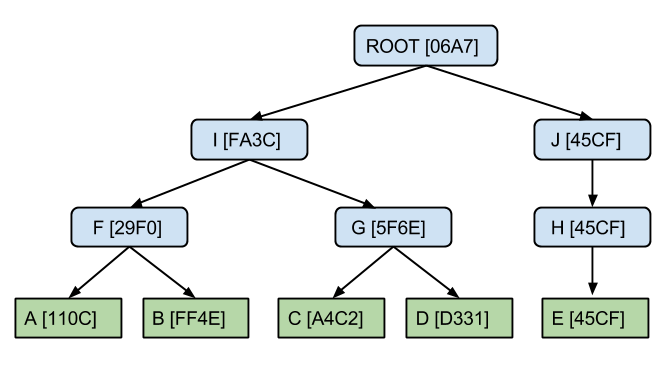
\includegraphics[scale=0.55]{merkle}}
\\
As shown in the example, each pair of (leaf) hash values are hashed together to construct a root hash. Eventually, a root of the tree is computed, which is the root of the merkle tree.\\
\\ 
\textbf{\large{2. Nonce Computation (Proof of Work) \cite{merkle2}}}\\ 
\\ 
The proof of work used in Bitcoin takes advantage of the apparently random nature of cryptographic hashes. A good cryptographic hash algorithm converts arbitrary data into a seemingly-random number. If the data is modified in any way and the hash re-run, a new seemingly-random number is produced, so there is no way to modify the data to make the hash number predictable. To prove you did some extra work to create a block, you must create a hash of the block header which does not exceed a certain value. This certain value is a hash beginning with a predefined number of 0's in the case of Bitcoin's Blockchain . For example, if the maximum possible hash value is $2^{256} -1$ (this maximum value possible is also known as the Blockchain's difficulty), you can prove that you tried up to two combinations by producing a hash value less than $2^{255}$.\\
\\
\textbf{\large{3. Blocks' Creation\cite{merkle2}}}\\
\\
The root of the merkle tree is stored in the block header, which also contains the hash of the previous block header, to ensure that a modification in a block will also change the other blocks.\\
\hspace*{-1.25cm}{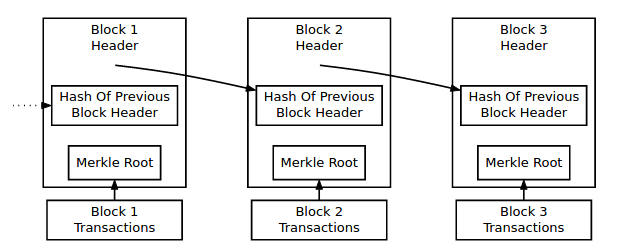
\includegraphics[scale=0.65]{merkle2}} 
\\   
Transactions are also chained together. Each transaction spends the satoshis previously received in one or more earlier transactions, so the input of one transaction is the output of a previous transaction. \\
A single transaction can create multiple outputs, as would be the case when sending to multiple addresses, but each output of a particular transaction can only be used as an input once in the blockchain. Any subsequent reference is a forbidden double spend—an attempt to spend the same satoshis twice.
\newpage
\hspace*{-0.75cm}{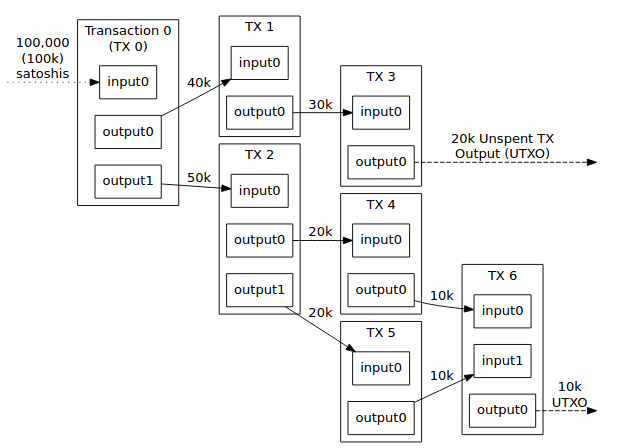
\includegraphics[scale=0.65]{merkle3}} 
\\   
Outputs are tied to transaction identifiers (TXIDs), which are the hashes of signed transactions. Because each output of a particular transaction can only be spent once, the outputs of all transactions included in the block chain can be categorized as either Unspent Transaction Outputs (UTXOs) or spent transaction outputs. For a payment to be valid, it must only use UTXOs as inputs.\\
New blocks will only be added to the block chain if their hash is at least as challenging as a difficulty value expected by the consensus protocol. Every 2,016 blocks, the network uses timestamps stored in each block header to calculate the number of seconds elapsed between generation of the first and last of those last 2,016 blocks. The ideal value is 1,209,600 seconds (two weeks). If it took fewer than two weeks to generate the 2,016 blocks, the expected difficulty value is increased proportionally (by as much as 300\%), so that the next 2,016 blocks should take exactly two weeks to generate if hashes are checked at the same rate. If it took more than two weeks to generate the blocks, the expected difficulty value is decreased proportionally (by as much as 75\%) for the same reason. Because each block header must hash to a value below the set difficulty, and because each block is linked to the block that preceded it, it requires (on average) as much hashing power to propagate a modified block as the entire Bitcoin network expended between the time the original block was created and the present time. Only if you acquired a majority of the network’s hashing power could you reliably execute such a 51 percent attack against transaction history (although, it should be noted, that even less than 50\% of the hashing power still has a good chance of performing such attacks).
\newpage
\section{Problem Domain}
Although the previous section contained a specific SFC security approach, we've chosen to define the problem domain for our work from a general security perspective. This change of perspective was by no means a random choice of ours, but it was rather due to the fact that Service Function Chains applications are still under continuous development, which makes it even harder to choose a specific SFC use case for security, or even focusing on a SFC plane to secure. This new SFC development on the cloud market become obvious when we look at the "established" NFV platforms that are supposed to provide SFC services. For instance, Openstack, a major leader in the IaaS (Infrastructure as a Service) market, still doesn't give a "stable" solution in terms of SFC. In spite of the promising signs that Openstack is showing in "port chaining" in its networking component Neutron, and the current NFV platform main project Tacker, port chaining is more of a chain of classification than network function chain, as "Service VMs must be attached at points in the network and then traffic must be steered between these attachment points". On the other hand, Tacker, besides the fact of its limited documentation to basic applications, is still showing bugs when an adaptation of context is required for a specific use case (19 official bugs in 2017 as of the moment of writing of this report)\cite{bugs}. For all these reasons, we discuss the problem domain from the security three A's perspective: Authentication, Authorization, Accountability.  Authentication represents the ability to access  to the system, be it from actual users, components, traffic, or any participating entity of the system.  Authorization, however, specifies the functionalities that each entity has access to after getting authenticated by the system. Finally, accountability provides the feature of tracing/keeping the records of the different actions that are being performed within the system, allowing thereby to refer each action to the system's participant that has performed it. Therefore, accountability prove its massive usefulness after the system has been breached, or if it's simply not working correctly. In this work, we give various proposals regarding how the Blockchain technology can help in securing these three aspects in the Service Function Chains context. 
\subsection{Authentication}
Service Function Chains consists of interactions among various networking components, in order to decide eventually the path that the packets will follow and the service functions that will be applied upon them. Those interactions include the messages exchanged among the different components. Authenticating these messages can increase the security of the chain and ensure that it is functionning rightfully. A hash of each message can be computed and stored in the blockchain. Components can check the blockchain after receiving a message, then they would simply compare of the hashes to prove the authenticity of the message. A case for authentication in the blockchain can also be made for the interfaces, components and devices participating in the SFC.
\subsection{Authorization}
Defining different levels of authorization and privileges using blockchain is not as obvious as it may seem. A potential implementation of this feature using the blockchain technology may be done with the public and permissionned blockchains, in an architecture where the participants in the public blockchain may have only reading rights and consulting the contents of the chain, while another private/permissioned chain is made for the participants that can contribute in writing blocks within the chain.
\subsection{Accountability}
Using Blockchain for accountability is probably the most fitting use case in the SFC context. Blockchains are naturally used in Bitcoins to keep record of transactions. There is also various blockchain applications for copyrights \cite{copyrights}, digital signatures and verification \cite{blocksign}, and health care records \cite{health}. If anything, it only shows how the blockchain is used for keeping immutable records in different contexts. Likewise, blockchain could be deployed in Service Function Chains to keep records and logs of what is performed inside the chain: exchange of messages, classification rules' update, change of paths for some Service Functions...etc. Blockchain will not ensure only keeping the records inside the chain, but it will guarantee their integrity as well, since those records are being witnessed by the multiple participants within the chain and stored in the distributed ledger, allowing thereby safe monitoring of the SFC and knowing exactly who did what.
\subsection{Conclusion}
In an ideal scenario, our work would have included the different potential use cases for securing Service Function Chains with Blockchain. However, this work is being accomplished during an internship, and is, consequently, limited by time constraints. Moreover, even if the future looks bright for Service Function Chains as well as Blockchain technology, they're still discussed in theory rather than put in place as real life applications \cite{sfc} \cite{btc}. Consequently, we've chosen to focus on accountability of the SFC using Blockchain technology, as keeping records is Blockchain's main use case, although it was introduced initially for financial transactions' use, this work will require adapting the technology for the service function chains context.
\newpage
\section{Overview Of Blockchain-Based Solutions For Records-Keeping}
Blockchain can be generally described as a distributed ledger linking numerous blocks of data in a sequenced manner, in order to keep track of the different transactions taking place within the system. The content of the ledger is being agreed on by all the participants in the system, through a distributed consensus algorithm, in which every participant is witnessing the transactions taking place and therefore proposing a block of transactions based on these witnesses. Although the principle is the same, different blockchain platforms choose different approaches (public/private, PoW/PoS,...) to implement this technology. This approach variation is mainly due to the application field (Finance, Health care, Copyrights protection,...) and what a developer may want to achieve with the blockchain technology stack. Although a benchmarking of the record keeping solutions would have presented immense profit for our cause, the big diversity of these solutions in terms of approach, the platform they lay upon and the target problem domain made it even harder for us to find a stable criteria for comparing the solutions and find out to what extent they fit for our SFC use case. Therefore, the remaining parts of this section offers simply an overview of multiple blockchain solutions that are mainly destinated to keep records in different contexts, with a display of their main characteristics and advantages.  
\subsection{Blockchain Platforms}
\textbf{\large{1.Bitcoin}}\\
\\
The first, and most famous blockchain platform.\enspace Launched in 2009 by the anonymous Satoshi Nakamoto, the blockchain technology was directly involved in making Bitcoin the most valued cryptocurrency up to date \cite{value}. The Bitcoin blockchain maintains the transactions' records made by the different participants in the Bitcoin network. It does also rely on the proof of work principle to prove the authenticity of the records. PoW is basically about solving a mathematical puzzle consisting of finding the right nonce. The "nonce" in a bitcoin block is a 32-bit (4-byte) field whose value is set so that the hash of the block will contain a run of leading zeros. the number of zeros is global variable in the Bitcoin network, and it changes after every 2016 blocks \cite{bitwiki}. Bitcoins are put into circulation by mining. Mining is “is the process of adding transaction records to Bitcoin's public ledger of past transactions or blockchain” \cite{mining}.\\
\\
\textbf{\large{2. Ethereum}}\\ 
\\
Relying on the same blockchain principles, ether (Ethereum-based cryptocurrency) is emerging as the second most successful digital currency behind bitcoins \cite{value}. Nevertheless, Ethereum was designed to be much more than a payment system.  It is "a decentralized platform that runs smart contracts: applications that run exactly as programmed without any possibility of downtime, censorship, fraud or third party interference" \cite{ethereum}.  Ethereum block times are currently at about 14 seconds, compared to Bitcoin’s 10 minutes. Ethereum also currently operates on a proof-of-work basis. Miners are rewarded for processing transactions and executing smart contracts, which create blocks.
\subsection{Blockchain-based record keeping solutions}
As interest in blockchain-based solutions -be it through companies or simple initiatives/projects- is growing dramatically \cite{trends}, many companies who are adopting this technology prefer to build their solutions either on the Bitcoin blockchain or the Ethereum blockchain \cite{canada}, given their well-established status as the two most successful Blockchain platforms currently \cite{value}. Therefore, the evaluation of the record keeping solutions in these section should take into account how these solutions are making profit from Bitcoin/Ethereum Blockchains to ensure the security of their records.\\
\\
\textbf{\large{Blockstack}}\\
\\
Originally a naming system which is built on Bitcoin's Blockchain, Blockcstack provides the ability of tracking key-value pairs in form of (unique) names and their associated data. In the Blockstack Whitepaper \cite{bswp}, there is another confirmation, after a handful of experiences, that the Bitcoin's Blockchain is probably the most secure Blockchain platform available currently. If that is partly due to the big network of participants in Bitcoin, the difficuly of controlling 51\% of the processing power inside the network,
where all the participants are even, is an important factor as well. On the other hand, Blockcstack developpers chose to take a different approach in terms of storage, given that the Bitcoin Blockchain can only hold data in the order of kilobytes \cite{satoshi}. Therefore, Blockcstack uses blockchain "as a communication channel for announcing state changes, as any changes to the state of name-value pairs can only be announced in new blockchain blocks" \cite{bswp}. As for storing these records of the name-data pairs, Blockstack uses a dedicated data plane for that purpose.\\
\\
\textbf{\large{Proof of Existence \cite{poe}}}\\
\\ 
An online service for storing and timestamping the existence of a document inside the blockchain. This secure storage is done traditionnaly by keeping a hash of the file in the chain, with a referrence also to the time in which the document was stored. Consequently, such mechanism does not only ensure that the files' content cannot be seen by the Bitcoin's network participants (since PoE is built on Bitcoin's Blockchain), it allows also validating the document's existence "even if this site (proofofexsitence.com) is compromised or down". On the technical aspect, it is worth noting that this  solution also uses the OP\_RETRUN field to pass specific information with the transaction. To confirm a document's existence at a certain timestamped time, checking the OP\_RETURN field in blockchain trasancations for the SHA-256 hash of the document, prepended by the PoE marker bytes (0x444f4350524f4f46) should be sufficient. The existence of that transaction in the blockchain proves the existence of the document at the timpestamped time.\\
\\
\textbf{\large{Hyperledger}}\\
\\
Even though we stated earlier that most current well-established solutions are either Bitcoin or Ethereum based, Hyperledger succeeded to make a name for itself as a smart contract blockchain platform, relying on a somewhat different approach. Initiated by The Linux Foundation, Hyperledger started a set of distributed ledger solutions based on different platforms and programming languages. Hyperledger is based on the expectation that there will be many blockchain networks, with each network ledger serving a different goal \cite{hype}. In this section, we present the Hyperledger Blockchain explorer, and then we take a keen interest on Hyperledger Fabric.
\\
\\
\textbf{\large{1. Hyperledger Blockchain Explorer}}\\
\\
A blockchain explorer web application. It allows "to view/query blocks, transactions and associated data, network information (name, status, list of nodes), chain codes/transaction families (view/invoke/deploy/query) and any other relevant information stored in the ledger" \cite{hyperledger}
\\
\\
\textbf{\large{2. Hyperledger Fabric}}\\
\\
Hyperldger Fabric is simply "a permissioned blockchain platform aimed at business use. It is open-source and based on standards, runs user-defined smart contracts, supports strong security and identity features, and uses a modular architecture with pluggable consensus protocols" \cite{hyper}. It aims to advance blockchain technology by identifying and realizing a cross-industry open standard platform for distributed ledgers, which can transform the way business transactions are conducted globally. Generally, Hyperledger Fabric offers the major advantage of ensuring private transactions/contracts between sinlge nodes in a network of nodes. This is made possible through providing 
private communication channels between participants. Therefore, any two (or more) participating nodes can share their own distributed ledger, containing their own private transactions, with the rest of the network being unaware of this private ledger. As for the participating peers in the network, the fabric distinguishes between two kinds of peers: A validating peer is a node on the network responsible for running consensus, validating transactions, and maintaining the ledger. On the other hand, a non-validating peer is a node that functions as a proxy to connect clients (issuing transactions) to validating peers. A non-validating peer does not execute transactions but it may verify them \cite{hyper}. the smart contracts run by Hyperledger Fabric are written in Go language, and they are called chaincode. The transactions' operations are generally divided into 3 categories\\
\begin{enumerate}
\item \textbf{Deploy} Allows traditional deployment of smart contracts, as this operation installs the chaincode taken as its input in the peers of the network. After the deployment, the chaincode can be invoked by the different peers.
\item \textbf{Invoke} Provide the ability to invoke a transaction of a particular chaincode that has been installed earlier through a deploy transaction \cite{hyper}. Depending on the arguments taken by the operation; the chaincode defines the type and executes the
transaction, may read and write entries in its state accordingly, and indicates whether it succeeded or
failed.
\item \textbf{Query} Returns an entry of the state directly from reading the peer’s persistent state \cite{hyper}.
\end{enumerate}
\textbf{\large{Namecoin \cite{namecoin}}}\\
\\
Just like Blockstack, Namecoin is another blockchain based solution for namespaces' storage. Relying on forking the Bitcoin's blockchain (using Bitcoin's blockchain itself for specific purposes and additional functions), Namecoin allows secure storage of key value pairs, ensuring consequently the uniqueness of names inside the blockchain. On the other hand, the values associated to different namespaces aren't necessarily unique, as the same value can exist within different namespaces. For the additionnal functions, Namecoin introduced three new operations: \textbf{NAME\_ NEW} which allows a client to choose a name (if it's not already taken), \textbf{NAME\_ FIRSTUPDATE} takes as input the output of the previous operation, and allows the client to associate initial values to the chosen name and \textbf{NAME\_ UPDATE}  takes as input the output of NAME\_ FIRSTUPDATE and gives the client the possibility to change or insert new values in the name that he has chosen.
\newpage
\section{Blockchain Record-Keeping with Bitcoin's \\OP\_RETURN}
After doing an overview of various blockchain-based solutions for record-keeping, we present, in this section, a detailed explanation of our chosen solution for securing Service Function Chains using Bitcoin’s Blockchain. We focus on the accountability
of SFC, relying on the OP\_RETURN field of blockchain’s transactions to transmit the different messages exchanged between the SFC components,
ensuring therefeore immutable logging of the interactions that occur inside a Service Function Chain.
\section{Introduction}
Accountability, the third A in the famous security 3 A's (Authentication, Authorization and Accountability), is a major feature that should be taken into account in any implementation of a securtiy system. Accountablity's importance does not only lay in providing records of the different exchanges between the system's components, but it does also allow identifying points and sources of failure when the system stops working as expected or suffers a performance degradation. In the SFC context, a Service Function may shut down, a Service Function Forwarder might equally struggle with forwarding packets due to an overload. Therefore, keeping records of the interactions happening within the system enusres the system is working as expected as well as its high availability. In the next section, we give a brief reminder of the blockchain's principle, then we explain in details how Bitcoin's blockchain can be used for record-keeping.
\subsection{Record-Keeping using Bitcoin's Blockchain}
Blockchain can be generally described as a distributed ledger that serves as a record keeper for transactions occuring among the different Bitcoin's network participants. By keeping records of these transactions, the peer to peer system ensures that assets (bitcoins) are not being double-spent. The general consensus protocol adopted by the blockchain allows the majority of participants to testify whether a transactions has effectively taken place or not. Eventually, a block of multiple transactions is confirmed every 10 minutes. Once a block get "chained" within the distributed ledger, it can never be changed or altered, or at least it will require taking down the majority of the computing power of the participants to change a confirmed block of the chain (51\% attack). Given this strength of the blockchain of keeping records and ensuring their authenticity, we figured out a use case where the Blockchain can be depolyed in the SFC context to keep records of the interactions occuring among the SFC components, and the meassages that are being exchanged within the Function Chain.
\subsection{OP\_RETURN field overview\cite{bit}}
In the early days of the Bitcoin, users and participants were not concerned how the underlying blockchain technology could be used in different contexts and for various use cases, as they were embracing the breakthrough of the digtal currency emergence. As it started to get popular and gained momentum, IT developers proposed applications for the blockchain outside the finance industry: Keeping records for healthcare, Legal possession of assets, Copyrights...etc. Such applications would usually require sending/receiving different kind of messages with the transaction (confirmation, acknowledgement of receipt among others). As a consequence, developers used one way or another to get the messages sent with the transaction. Back in 2013 different players in the bitcoin ecosystem were trying to include bits of information into transactions so that they could take advantage of the irreversibility of the blockchain. Imagine, for instance, you wanted to write a contract and place it in an unchangeable location that at any future date one could go back to verify it existed. You can do this by using the blockchain. You add some bits to the transaction's scriptSig value that don't alter the end result of running that script, but allow you to store information like "I hereby declare to give asset A to address XYZ at time UNIX\_TIMESTAMP". There were even stranger ways people would add extra bits, like including it in the BTC value of an output. Some members of the community did not like this, as they saw these extra bits as polluting the blockchain. The extra bits were a network efficiency concern because more bits meant larger block chains and more of an onus on those who are running full nodes, and it was also a community consensus concern because they thought "we all implicitly agreed to store financial data in the blockchain, which is important to everyone, but we did not agree to store data like small text messages and invoice text". To reach a middle ground in these opposing views, the core-developers made the opcode OP\_RETURN a valid opcode to be used in a bitcoin transaction, which allows 80 arbitrary bytes to be used in an unspendable transaction. Later in February 2014, the bytes count was reduced from 80 to 40 bytes. On 16 Nov 2014 there was a pull request to have the OP\_RETURN size increased “back” to 80. This was then accepted (merged) on 4 Feb 2015 \cite{bit2}.\\
To gain deeper knowledge about OP\_RETURN transactions in practice, we made a transaction in Bitcoin's testnet containing "Hello, testnet!" in its OP\_RETURN field. We've use the online Bitcoin's explorer \url{https://www.blocktrail.com}, which allowed to check the transaction's fields once it got confirmed inside a Bitcoin's block. The figures below show the transaction's details in Bitcoin's core and its fields in the Blockchain's explorer.
\\
\\
\hspace*{1cm}{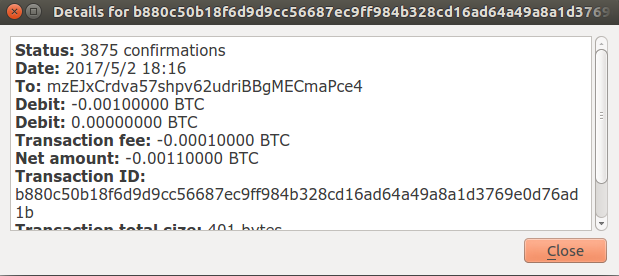
\includegraphics[scale=0.55]{op1}}
\\
\\
\hspace*{-0.1cm}{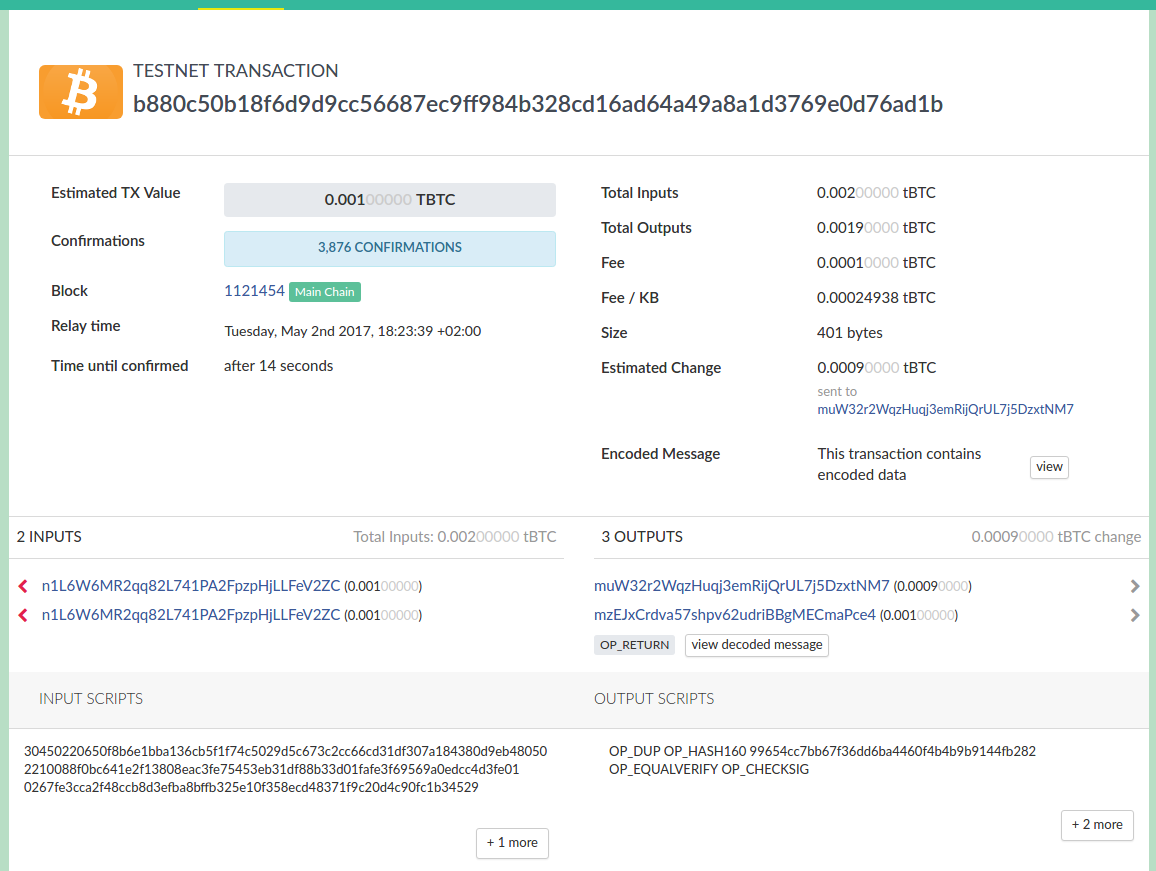
\includegraphics[scale=0.35]{op2}}
\\
\\
\hspace*{3cm}{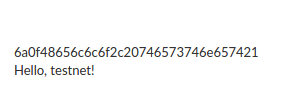
\includegraphics[scale=0.75]{op3}}
\\
In the above figure, on top there is the hex message contained in the OP\_RETURN field of the transaction. The first hex value (0x6a) is the OP\_RETURN opcode in Bitcoin's stack-based programming language \cite{wikik}. The second hex value (0x0f) refers to the number of bytes of the actual message.  Therefore, our message only used 15 bytes (0x0f equals 15) of the 80 bytes offered by the OP\_RETURN field. As shown in the figure below, translating the remaining part of the hexadecimal message to ASCII language results in the expected "Hello, tesnet!" message.
\\
\\
\hspace*{1cm}{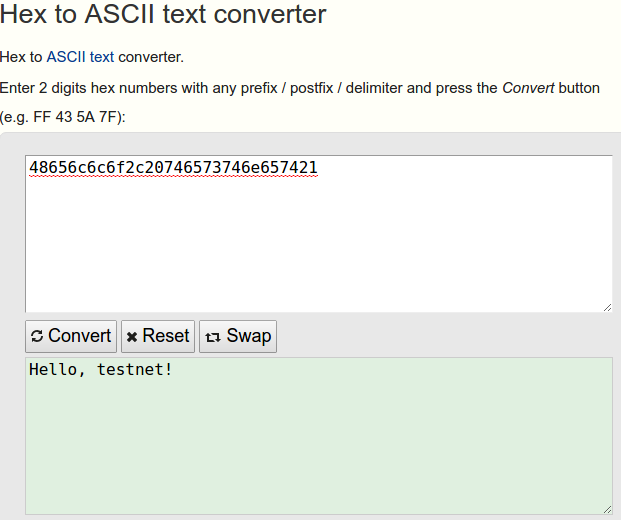
\includegraphics[scale=0.55]{op4}}
\\  

\subsection{Constraints}
Even though using OP\_RETURN for transmitting (and eventually storing) the exchanged messages inside a Service Function Chain seems like a good and equally innovative option, this solution would not be implemented without any constraints to be taken into account. The network overload could be problematic, since extra data will have to be carried within transaction packets on a regular basis. As a consequence, packets' fragmentation maybe required to ensure the overall network performance doesn't suffer a degradation. Moreover, logs' storage should also be thought about carefully, and finding the most adequate storage solution for this use case might present another problem. A solution that may be possible is finding an external storage deposit that interacts with the SFC and bitcoin network via an API. The details of the  proposed solutions should depend on the implementation and the used platforms.  













